\chapter{Laboratorium 2}
\label{cha:Lab002}
\makeatletter


% *********************************************************************
% w poniższej metryczce należy uzupełnić informacje o:
% - temacie ćwiczenia
% - numer ćwiczenia
% - numer grupy laboratoryjnej
% - numer zespołu
% - datę wykonania ćwiczenia oraz oddania ćwiczenia.
% *********************************************************************

\begin{table}[H]
    \centering
    \renewcommand{\tabularxcolumn}[1]{m{#1}}  % Dostosowanie kolumny do zawartości
    \newcolumntype{C}{>{\centering\arraybackslash}X}
    \begin{tabularx}{\linewidth}{|C|C|}
        \hline
        \multicolumn{2}{|c|}{\makecell{\textbf{\Large{Biometryczne Systemy Zabezpieczeń}} \\ \textbf{Ćwiczenia Laboratoryjne}}} \\ \hline
        \multicolumn{1}{|l|}{Temat}                    &              DETEKCJA KRAWĘDZI W OBRAZIE METODAMI SPLOTOWYMI.            \\ \hline
        \multicolumn{1}{|l|}{Ćwiczenie nr:}                    &      02                   \\ \hline
        \multicolumn{1}{|l|}{Autorzy:}                         &   \@author                              \\ \hline
        \multicolumn{1}{|l|}{Grupa laboratoryjna}                       &       02               \\ \hline
        \multicolumn{1}{|l|}{Zespół nr. }                       &    XX                  \\ \hline
        \multicolumn{1}{|l|}{Data wykonana ćwiczenia}         &  26.04.2025     \\ \hline
        \multicolumn{1}{|l|}{Data oddania ćwiczenia  }         &   13.05.2025     \\ \hline
    \end{tabularx}
\end{table}


\section{Cel ćwiczenia}

Filtracja splotowa to jedno z podstawowych narzędzi przetwarzania obrazów, wykorzystywane do wygładzania, wykrywania krawędzi, redukcji szumów oraz innych operacji poprawiających jakość obrazu. Splot (ang. convolution) polega na przekształceniu obrazu poprzez nałożenie na niego maski (jądra) filtrującego. Celem laboratorium jest implementacja algorytmu splotowego w MATLAB-ie oraz zbadanie wpływu różnych filtrów na obraz.

\section{Wstęp teoretyczny}

\subsubsection{Filtracja splotowa}

Filtracja splotowa (ang. convolution filtering) jest podstawową metodą przetwarzania obrazów w dziedzinie przestrzennej. Polega ona na nakładaniu na obraz niewielkiej maski (kernela) i obliczaniu nowych wartości pikseli jako sumy ważonej sąsiednich pikseli zgodnie z wartościami w masce. W praktyce oznacza to, że dla każdego punktu obrazu uwzględnia się przyległe piksele, których wartości mnoży się przez odpowiadające wagi z maski, a następnie sumuje. Taki proces pozwala uzyskać różne efekty – od wygładzania (rozmycia) poprzez wyostrzanie po detekcję krawędzi, w zależności od przyjętych wag w masce filtra.

\subsubsection{Filtry krawędziowe (Roberts, Prewitt, Sobel, Laplace)}

Operator Robertsa – jest jednym z pierwszych detektorów krawędzi wykorzystujących maski różnicowe. Używa dwóch małych masek 2×2 do przybliżenia gradientu obrazu w kierunkach ukośnych. Filtr ten jest bardzo prosty obliczeniowo (maski zawierają tylko liczby całkowite), jednak jego wadą jest duża wrażliwość na szum. Wynikiem działania operatora Robertsa są zmiany intensywności wzdłuż przekątnych, co prowadzi do wykrywania krawędzi o orientacji diagonalnej.

Operator Prewitta – wykorzystuje dwie maski 3×3 do przybliżenia pochodnych obrazu w kierunku poziomym i pionowym. Każda z masek jest wynikiem splotu filtru różnicującego z filtrem uśredniającym. Dzięki temu operator Prewitta częściowo wygładza obraz, co poprawia wykrywanie krawędzi poziomych i pionowych. Generowany wektor gradientu obrazu wskazuje siłę krawędzi (długość wektora) oraz jej orientację (kierunek wektora).

Operator Sobela – podobnie jak Prewitt, używa masek 3×3, jednak nadaje większe wagi środkowym elementom masek (wartość 2), co skutkuje silniejszym wygładzeniem i zwiększoną odpornością na szum. Operator Sobela wydajnie przybliża gradient intensywności obrazu, szczególnie eksponując miejsca gwałtownych zmian jasności.

Operator Laplace’a – oparty jest na drugiej pochodnej obrazu (Laplasjanie) i wykrywa zmiany intensywności niezależnie od kierunku. Jest to filtr drugiego rzędu, izotropowy w przestrzeni 2D. Operator Laplace’a uwypukla obszary szybkiej zmiany jasności, ale jest również podatny na szumy. Charakterystyczną cechą wyników Laplasjanu jest wykrywanie miejsc przecięcia zera (zero-crossings), które odpowiadają lokalizacjom krawędzi.

\subsubsection{Filtr medianowy a filtr uśredniający}

Filtr medianowy jest nieliniowym filtrem, w którym wartość piksela zastępowana jest medianą wartości z sąsiadujących pikseli. Dzięki temu skutecznie usuwa szum impulsowy typu „sól i pieprz”, zachowując jednocześnie ostrość krawędzi. W przeciwieństwie do filtrów liniowych, filtr medianowy nie wprowadza nowych wartości spoza przedziału istniejących intensywności, co zapobiega powstawaniu artefaktów.

Filtr uśredniający (średnia arytmetyczna) jest filtrem liniowym, który zastępuje wartość piksela średnią z jego sąsiadów. Filtr ten skutecznie redukuje szumy o rozkładzie Gaussa, jednak prowadzi do rozmycia krawędzi i utraty szczegółów. W praktyce filtr medianowy jest preferowany do usuwania szumu impulsowego, natomiast filtr uśredniający stosuje się głównie do ogólnego wygładzania obrazu.

\subsubsection{Szum typu „sól i pieprz” (impulsowy)}

Szum typu „sól i pieprz” to rodzaj szumu impulsowego, w którym losowe piksele przyjmują wartości minimalne (0, „pieprz”) lub maksymalne (255, „sól”). Zazwyczaj występuje na skutek błędów transmisji, uszkodzeń matrycy detektora lub błędów zapisu danych. Do jego usunięcia najlepiej nadają się filtry medianowe, które skutecznie eliminują pojedyncze anomalie bez znaczącej utraty ostrości obrazu. Filtry liniowe, takie jak filtr uśredniający, są mniej skuteczne, ponieważ rozmywają szum na większe obszary obrazu.

\section{Opis wykorzystywanego oprogramowania i narzędzi}

Do przeprowadzenia eksperymentu wykorzystano środowisko MATLAB oraz bibliotekę Image Processing Toolbox. Kluczowe funkcje używane w analizie to:

\begin{itemize}
	\item \texttt{imfilter()} – funkcja MATLAB służąca do filtracji obrazów za pomocą splotu lub korelacji z podaną maską. Pozwala na wybór sposobu obramowania granic obrazu oraz zachowuje typ danych wejściowych. Funkcja \texttt{imfilter()} umożliwia wygodne operacje na obrazach, zachowując ich oryginalne rozmiary.
	
	\item \texttt{conv2()} – funkcja realizująca dwuwymiarowy klasyczny splot, domyślnie zwracająca wynik o większym rozmiarze niż obraz wejściowy. Wynikowy obraz jest typu zmiennoprzecinkowego (double). \texttt{conv2()} jest wydajniejsza dla dużych masek, jednak wymaga ręcznego dostosowania rozmiaru i rzutowania typu wynikowego.
\end{itemize}
\clearpage

\section{Zadania do wykonania samodzielnego}

\subsection{Zadanie 1}

\subsubsection{Treść}
\textbf{Filtrowanie splotowe obrazu oka:}

Wykorzystując dowolny obraz biometryczny tęczówki oka wykonaj program dokonujący
filtracji splotowej filtrami Robertsa, Prewitta, Sobela oraz Laplace’a. Uwzględnij w programie
możliwość zadawania rozmiaru maski kernela 3x3 oraz 5x5.

\begin{itemize}
	\item Wyświetl wyniki filtracji w oknie wykorzystując funkcję subplot.
	\item Porównaj efekty filtracji dla różnych filtrów. Sprawdź wpływ zmiany rozmiaru maski filtra na
	wynik końcowy.
	\item Wprowadź do obrazu zadaną porcję szumu SaltAndPepper wykorzystując funkcję imnoise.
	\item Przeprowadź na obrazie wejściowym filtrację medianową i uśredniającą a następnie porównaj otrzymane wyniki. Ponów procedurę wykrycia krawędzi w obrazie; przedstaw w sprawozdaniu dyskusję otrzymanych wyników.
	\item Wczytaj obraz kolorowy (peppers.png) i zastosuj filtrację na każdej składowej R, G, B osobno.
	Połącz przefiltrowane składowe w nowy obraz i wyświetl wynik.
	\item Sprawdź, jak działa imfilter(I, h, 'same') w porównaniu do conv2(). Czy wyniki są identyczne?
	Jakie są różnice?
\end{itemize}

\subsubsection{Przykładowy program}

\lstinputlisting[style= matlabStyle, caption= Wczytanie obrazu i stworzenie konwersji, label=Lab002_l1]{src/Lab002/zadanie1.m}

\subsubsection{Obrazy}

\begin{figure}[H]
	\centering
	\begin{subfigure}[t]{0.45\linewidth}
		\centering
		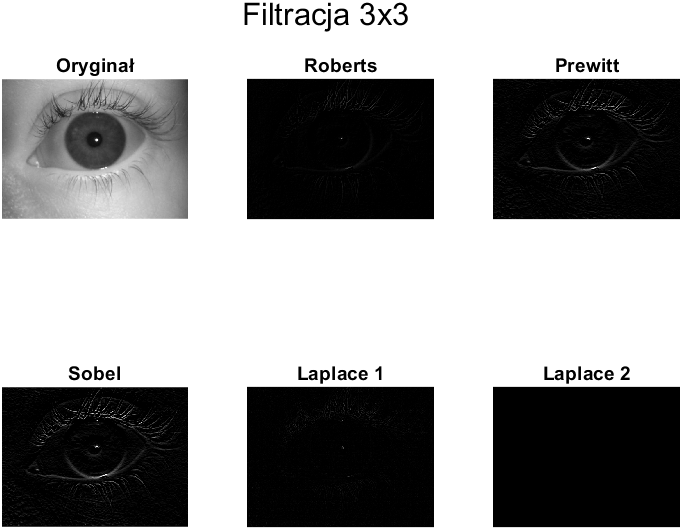
\includegraphics[width=\linewidth]{src/Lab002/zadanie1images/filtracja_3x3.png}
		\caption{Filtracja splotowa 3x3}
		\label{fig:3x3}
	\end{subfigure}
	\hfill
	\begin{subfigure}[t]{0.45\linewidth}
		\centering
		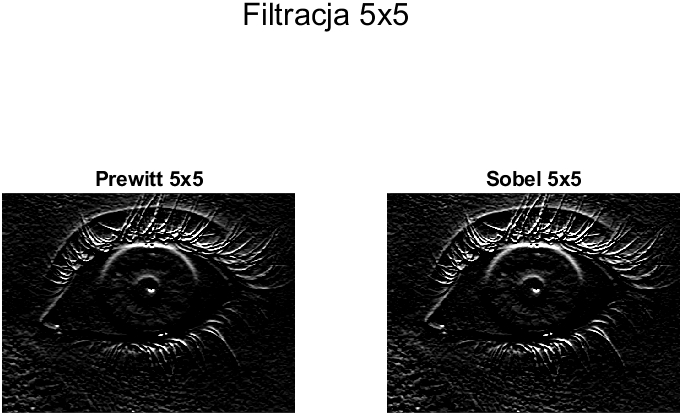
\includegraphics[width=\linewidth]{src/Lab002/zadanie1images/filtracja_5x5.png}
		\caption{Filtracja splotowa 5x5}
		\label{fig:5x5}
	\end{subfigure}

	\begin{subfigure}[t]{0.45\linewidth}
		\centering
		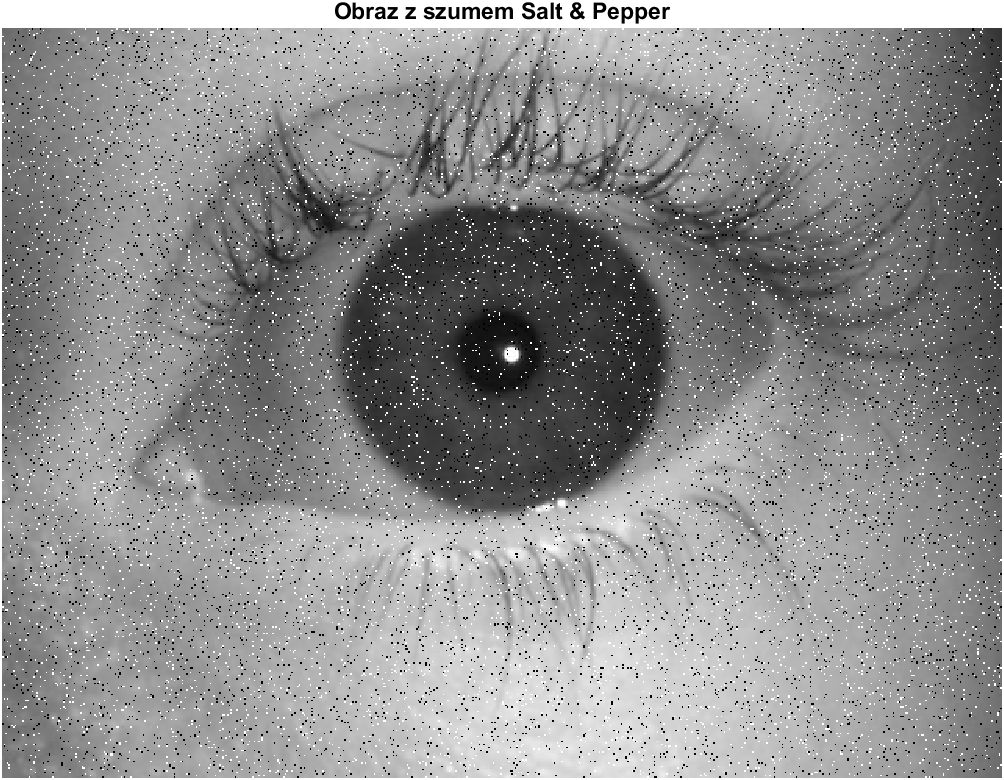
\includegraphics[width=\linewidth]{src/Lab002/zadanie1images/szum_salt_pepper.png}
		\caption{Obraz z szumem Salt and Pepper}
		\label{fig:SaltNPepper}
	\end{subfigure}
	\hfill
	\begin{subfigure}[t]{0.45\linewidth}
		\centering
		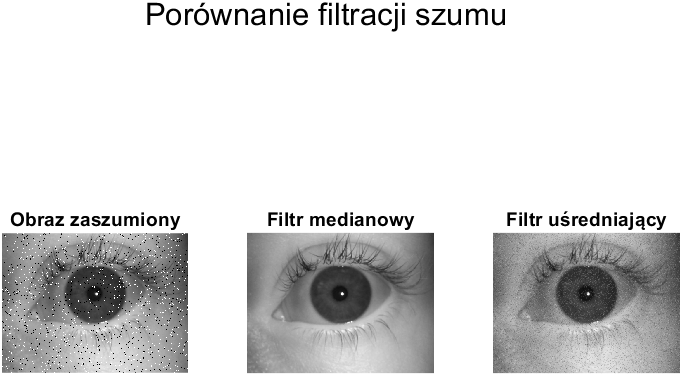
\includegraphics[width=\linewidth]{src/Lab002/zadanie1images/filtracja_szumu.png}
		\caption{Filtracja medianowa i uśredniająca}
		\label{fig:filteringMU}
	\end{subfigure}
	
	\begin{subfigure}[t]{0.45\linewidth}
		\centering
		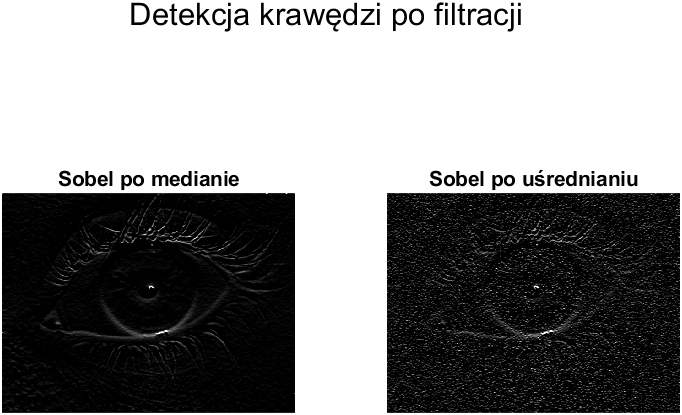
\includegraphics[width=\linewidth]{src/Lab002/zadanie1images/detekcja_krawedzi_po_filtracji.png}
		\caption{Detekja po filtracji}
		\label{fig:AfterFiltering}
	\end{subfigure}
	\hfill
	\begin{subfigure}[t]{0.45\linewidth}
		\centering
		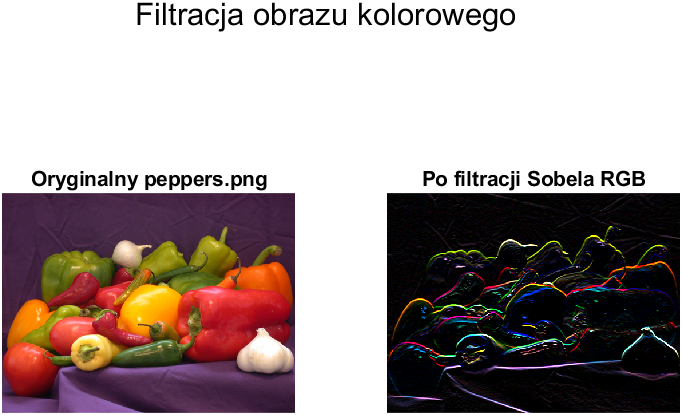
\includegraphics[width=\linewidth]{src/Lab002/zadanie1images/filtracja_rgb.png}
		\caption{Filtracja obrazu kolorowego}
		\label{fig:filtracja_rgb}
	\end{subfigure}

	\begin{subfigure}[t]{0.45\linewidth}
		\centering
		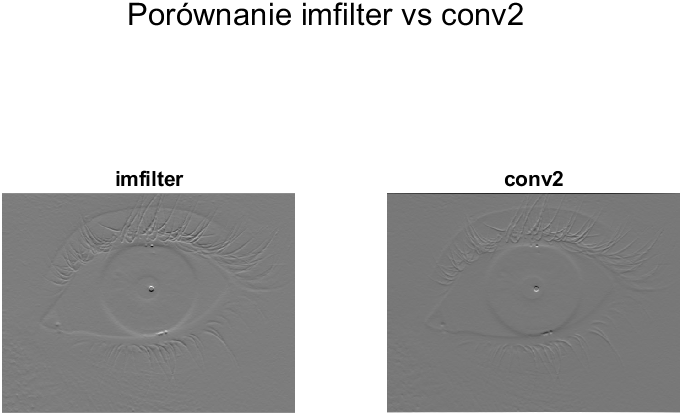
\includegraphics[width=\linewidth]{src/Lab002/zadanie1images/porownanie_imfilter_conv2.png}
		\caption{Porównanie imfilter i conv2}
		\label{fig:Imfilter_Conv2}
	\end{subfigure}
	
	\caption{Wizualizacja obrazów w różnych filtracjach splotowych.}
	\label{fig:lab002_images1}
\end{figure}

\section{Wnioski}
Na podstawie przeprowadzonych eksperymentów można stwierdzić, że:

\begin{itemize}
	\item \textbf{Filtry krawędziowe (Roberts, Prewitt, Sobel, Laplace)} skutecznie wykrywają zmiany intensywności w obrazie, jednak ich charakterystyka znacząco się różni. Operator Robertsa jest prosty i szybki obliczeniowo, lecz wykazuje dużą wrażliwość na szum i słabo radzi sobie z krawędziami innymi niż ukośne. Operator Prewitta oraz Sobela są bardziej odpornymi filtrami, przy czym filtr Sobela oferuje lepsze wygładzenie dzięki większemu obciążeniu środkowych pikseli. Operator Laplace’a umożliwia wykrycie krawędzi niezależnie od kierunku, ale jego wrażliwość na szumy jest jeszcze większa niż filtrów pierwszorzędowych.
	
	\item \textbf{Rozmiar maski filtra} wpływa na wynik filtracji: maski 5x5 zapewniają mocniejsze wygładzanie i bardziej rozmyte krawędzie w porównaniu do masek 3x3. Zwiększenie rozmiaru maski powoduje, że filtr staje się mniej czuły na drobne detale i szum, ale za to mniej precyzyjnie lokalizuje krawędzie.
	
	\item \textbf{Wpływ szumu Salt\&Pepper} na jakość obrazu jest znaczny. Obecność tego typu zakłóceń prowadzi do licznych, losowych zaburzeń w obrazie, które mogą zostać błędnie zinterpretowane jako krawędzie podczas procesu filtracji.
	
	\item \textbf{Filtr medianowy} wykazuje wysoką skuteczność w usuwaniu szumu typu Salt\&Pepper przy zachowaniu krawędzi oraz struktury obrazu. W przeciwieństwie do niego, \textbf{filtr uśredniający} rozmywa obraz, prowadząc do rozmycia granic i mniejszej skuteczności w eliminacji impulsowych zakłóceń.
	
	\item \textbf{Filtracja obrazu kolorowego} (na osobnych kanałach RGB) umożliwia skuteczne przetwarzanie obrazów wielokanałowych. Jednak filtracja niezależnie każdego kanału może prowadzić do powstania artefaktów kolorystycznych, zwłaszcza w obszarach o silnych zmianach koloru.
	
	\item \textbf{Porównanie funkcji imfilter oraz conv2} wykazało, że obie metody dają podobne wyniki przy odpowiednim doborze opcji (parametr \texttt{'same'}). Funkcja \texttt{imfilter} jest bardziej elastyczna, oferując możliwość wyboru metody obsługi brzegów obrazu oraz zachowania typu danych. Z kolei \texttt{conv2} jest bardziej „surowa” i wymaga ręcznego dostosowania typu i rozmiaru wyniku.
\end{itemize}

Podsumowując, odpowiedni dobór metody filtracji, rozmiaru maski oraz sposobu redukcji szumów ma kluczowe znaczenie dla skutecznej analizy obrazów biometrycznych i przetwarzania obrazów cyfrowych w ogóle.
